% Created by tikzDevice version 0.12.6 on 2026-10-26 12:42:46
% !TEX encoding = UTF-8 Unicode
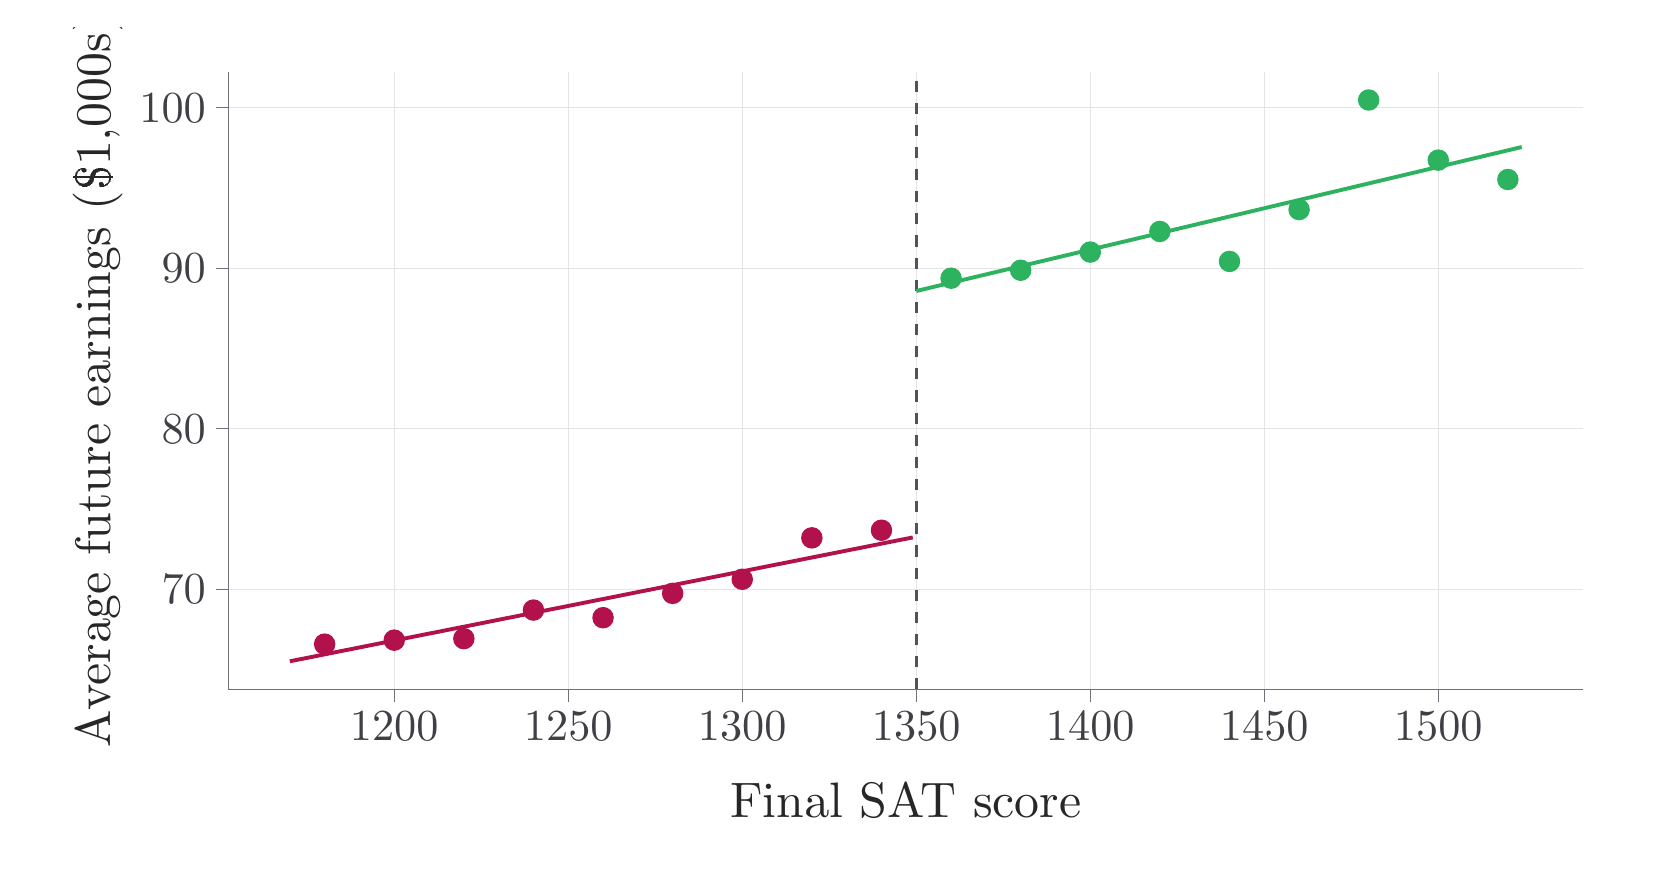
\begin{tikzpicture}[x=1pt,y=1pt]
\definecolor{fillColor}{RGB}{255,255,255}
\path[use as bounding box,fill=fillColor] (0,0) rectangle (578.16,303.53);
\begin{scope}
\path[clip] (  0.00,  0.00) rectangle (578.16,303.53);
\definecolor{drawColor}{RGB}{255,255,255}

\path[draw=drawColor,line width= 0.9pt,line join=round,line cap=round,fill=fillColor] (  0.00,  0.00) rectangle (578.16,303.53);
\end{scope}
\begin{scope}
\path[clip] ( 72.48, 64.43) rectangle (562.16,287.53);
\definecolor{drawColor}{RGB}{255,255,255}
\definecolor{fillColor}{RGB}{255,255,255}

\path[draw=drawColor,line width= 0.9pt,line join=round,line cap=round,fill=fillColor] ( 72.48, 64.43) rectangle (562.16,287.53);
\definecolor{drawColor}{RGB}{228,228,231}

\path[draw=drawColor,line width= 0.4pt,line join=round] ( 72.48,100.64) --
	(562.16,100.64);

\path[draw=drawColor,line width= 0.4pt,line join=round] ( 72.48,158.65) --
	(562.16,158.65);

\path[draw=drawColor,line width= 0.4pt,line join=round] ( 72.48,216.66) --
	(562.16,216.66);

\path[draw=drawColor,line width= 0.4pt,line join=round] ( 72.48,274.67) --
	(562.16,274.67);

\path[draw=drawColor,line width= 0.4pt,line join=round] (132.46, 64.43) --
	(132.46,287.53);

\path[draw=drawColor,line width= 0.4pt,line join=round] (195.34, 64.43) --
	(195.34,287.53);

\path[draw=drawColor,line width= 0.4pt,line join=round] (258.21, 64.43) --
	(258.21,287.53);

\path[draw=drawColor,line width= 0.4pt,line join=round] (321.09, 64.43) --
	(321.09,287.53);

\path[draw=drawColor,line width= 0.4pt,line join=round] (383.97, 64.43) --
	(383.97,287.53);

\path[draw=drawColor,line width= 0.4pt,line join=round] (446.84, 64.43) --
	(446.84,287.53);

\path[draw=drawColor,line width= 0.4pt,line join=round] (509.72, 64.43) --
	(509.72,287.53);
\definecolor{drawColor}{RGB}{82,82,91}

\path[draw=drawColor,line width= 1.1pt,dash pattern=on 4pt off 4pt ,line join=round] (321.09, 64.43) -- (321.09,287.53);
\definecolor{drawColor}{RGB}{179,17,75}
\definecolor{fillColor}{RGB}{179,17,75}

\path[draw=drawColor,line width= 0.6pt,line join=round,line cap=round,fill=fillColor] (132.46, 82.21) circle (  3.58);

\path[draw=drawColor,line width= 0.6pt,line join=round,line cap=round,fill=fillColor] (258.21,104.20) circle (  3.58);

\path[draw=drawColor,line width= 0.6pt,line join=round,line cap=round,fill=fillColor] (107.31, 80.77) circle (  3.58);

\path[draw=drawColor,line width= 0.6pt,line join=round,line cap=round,fill=fillColor] (233.06, 99.12) circle (  3.58);

\path[draw=drawColor,line width= 0.6pt,line join=round,line cap=round,fill=fillColor] (157.61, 82.76) circle (  3.58);

\path[draw=drawColor,line width= 0.6pt,line join=round,line cap=round,fill=fillColor] (182.76, 93.08) circle (  3.58);

\path[draw=drawColor,line width= 0.6pt,line join=round,line cap=round,fill=fillColor] (283.36,119.18) circle (  3.58);

\path[draw=drawColor,line width= 0.6pt,line join=round,line cap=round,fill=fillColor] (308.52,121.93) circle (  3.58);
\definecolor{drawColor}{RGB}{45,178,95}
\definecolor{fillColor}{RGB}{45,178,95}

\path[draw=drawColor,line width= 0.6pt,line join=round,line cap=round,fill=fillColor] (358.82,215.87) circle (  3.58);
\definecolor{drawColor}{RGB}{179,17,75}
\definecolor{fillColor}{RGB}{179,17,75}

\path[draw=drawColor,line width= 0.6pt,line join=round,line cap=round,fill=fillColor] (207.91, 90.32) circle (  3.58);
\definecolor{drawColor}{RGB}{45,178,95}
\definecolor{fillColor}{RGB}{45,178,95}

\path[draw=drawColor,line width= 0.6pt,line join=round,line cap=round,fill=fillColor] (409.12,229.89) circle (  3.58);

\path[draw=drawColor,line width= 0.6pt,line join=round,line cap=round,fill=fillColor] (383.97,222.44) circle (  3.58);

\path[draw=drawColor,line width= 0.6pt,line join=round,line cap=round,fill=fillColor] (333.67,213.00) circle (  3.58);

\path[draw=drawColor,line width= 0.6pt,line join=round,line cap=round,fill=fillColor] (434.27,219.06) circle (  3.58);

\path[draw=drawColor,line width= 0.6pt,line join=round,line cap=round,fill=fillColor] (484.57,277.39) circle (  3.58);

\path[draw=drawColor,line width= 0.6pt,line join=round,line cap=round,fill=fillColor] (459.42,237.80) circle (  3.58);

\path[draw=drawColor,line width= 0.6pt,line join=round,line cap=round,fill=fillColor] (509.72,255.67) circle (  3.58);

\path[draw=drawColor,line width= 0.6pt,line join=round,line cap=round,fill=fillColor] (534.87,248.66) circle (  3.58);
\definecolor{drawColor}{RGB}{179,17,75}

\path[draw=drawColor,line width= 1.4pt,line join=round] ( 94.73, 74.57) --
	( 97.58, 75.14) --
	(100.43, 75.70) --
	(103.28, 76.27) --
	(106.13, 76.84) --
	(108.98, 77.40) --
	(111.83, 77.97) --
	(114.68, 78.54) --
	(117.53, 79.10) --
	(120.38, 79.67) --
	(123.23, 80.23) --
	(126.08, 80.80) --
	(128.93, 81.37) --
	(131.78, 81.93) --
	(134.63, 82.50) --
	(137.47, 83.07) --
	(140.32, 83.63) --
	(143.17, 84.20) --
	(146.02, 84.77) --
	(148.87, 85.33) --
	(151.72, 85.90) --
	(154.57, 86.47) --
	(157.42, 87.03) --
	(160.27, 87.60) --
	(163.12, 88.17) --
	(165.97, 88.73) --
	(168.82, 89.30) --
	(171.67, 89.87) --
	(174.52, 90.43) --
	(177.37, 91.00) --
	(180.21, 91.57) --
	(183.06, 92.13) --
	(185.91, 92.70) --
	(188.76, 93.27) --
	(191.61, 93.83) --
	(194.46, 94.40) --
	(197.31, 94.97) --
	(200.16, 95.53) --
	(203.01, 96.10) --
	(205.86, 96.67) --
	(208.71, 97.23) --
	(211.56, 97.80) --
	(214.41, 98.37) --
	(217.26, 98.93) --
	(220.11, 99.50) --
	(222.96,100.07) --
	(225.80,100.63) --
	(228.65,101.20) --
	(231.50,101.77) --
	(234.35,102.33) --
	(237.20,102.90) --
	(240.05,103.46) --
	(242.90,104.03) --
	(245.75,104.60) --
	(248.60,105.16) --
	(251.45,105.73) --
	(254.30,106.30) --
	(257.15,106.86) --
	(260.00,107.43) --
	(262.85,108.00) --
	(265.70,108.56) --
	(268.54,109.13) --
	(271.39,109.70) --
	(274.24,110.26) --
	(277.09,110.83) --
	(279.94,111.40) --
	(282.79,111.96) --
	(285.64,112.53) --
	(288.49,113.10) --
	(291.34,113.66) --
	(294.19,114.23) --
	(297.04,114.80) --
	(299.89,115.36) --
	(302.74,115.93) --
	(305.59,116.50) --
	(308.44,117.06) --
	(311.29,117.63) --
	(314.13,118.20) --
	(316.98,118.76) --
	(319.83,119.33);
\definecolor{drawColor}{RGB}{45,178,95}

\path[draw=drawColor,line width= 1.4pt,line join=round] (321.09,208.37) --
	(323.86,209.03) --
	(326.63,209.69) --
	(329.40,210.35) --
	(332.17,211.01) --
	(334.94,211.67) --
	(337.71,212.33) --
	(340.48,212.98) --
	(343.25,213.64) --
	(346.02,214.30) --
	(348.79,214.96) --
	(351.56,215.62) --
	(354.33,216.28) --
	(357.10,216.94) --
	(359.87,217.59) --
	(362.64,218.25) --
	(365.41,218.91) --
	(368.18,219.57) --
	(370.95,220.23) --
	(373.72,220.89) --
	(376.49,221.55) --
	(379.26,222.20) --
	(382.03,222.86) --
	(384.80,223.52) --
	(387.56,224.18) --
	(390.33,224.84) --
	(393.10,225.50) --
	(395.87,226.16) --
	(398.64,226.81) --
	(401.41,227.47) --
	(404.18,228.13) --
	(406.95,228.79) --
	(409.72,229.45) --
	(412.49,230.11) --
	(415.26,230.77) --
	(418.03,231.42) --
	(420.80,232.08) --
	(423.57,232.74) --
	(426.34,233.40) --
	(429.11,234.06) --
	(431.88,234.72) --
	(434.65,235.38) --
	(437.42,236.03) --
	(440.19,236.69) --
	(442.96,237.35) --
	(445.73,238.01) --
	(448.50,238.67) --
	(451.27,239.33) --
	(454.04,239.99) --
	(456.81,240.64) --
	(459.58,241.30) --
	(462.35,241.96) --
	(465.12,242.62) --
	(467.89,243.28) --
	(470.66,243.94) --
	(473.43,244.60) --
	(476.20,245.25) --
	(478.97,245.91) --
	(481.74,246.57) --
	(484.51,247.23) --
	(487.28,247.89) --
	(490.05,248.55) --
	(492.82,249.21) --
	(495.59,249.86) --
	(498.36,250.52) --
	(501.13,251.18) --
	(503.89,251.84) --
	(506.66,252.50) --
	(509.43,253.16) --
	(512.20,253.81) --
	(514.97,254.47) --
	(517.74,255.13) --
	(520.51,255.79) --
	(523.28,256.45) --
	(526.05,257.11) --
	(528.82,257.77) --
	(531.59,258.42) --
	(534.36,259.08) --
	(537.13,259.74) --
	(539.90,260.40);
\end{scope}
\begin{scope}
\path[clip] (  0.00,  0.00) rectangle (578.16,303.53);
\definecolor{drawColor}{RGB}{113,113,122}

\path[draw=drawColor,line width= 0.3pt,line join=round] ( 72.48, 64.43) --
	( 72.48,287.53);
\end{scope}
\begin{scope}
\path[clip] (  0.00,  0.00) rectangle (578.16,303.53);
\definecolor{drawColor}{RGB}{63,63,70}

\node[text=drawColor,anchor=base east,inner sep=0pt, outer sep=0pt, scale=  1.60] at ( 64.38, 95.39) {70};

\node[text=drawColor,anchor=base east,inner sep=0pt, outer sep=0pt, scale=  1.60] at ( 64.38,153.40) {80};

\node[text=drawColor,anchor=base east,inner sep=0pt, outer sep=0pt, scale=  1.60] at ( 64.38,211.41) {90};

\node[text=drawColor,anchor=base east,inner sep=0pt, outer sep=0pt, scale=  1.60] at ( 64.38,269.42) {100};
\end{scope}
\begin{scope}
\path[clip] (  0.00,  0.00) rectangle (578.16,303.53);
\definecolor{drawColor}{RGB}{113,113,122}

\path[draw=drawColor,line width= 0.3pt,line join=round] ( 67.98,100.64) --
	( 72.48,100.64);

\path[draw=drawColor,line width= 0.3pt,line join=round] ( 67.98,158.65) --
	( 72.48,158.65);

\path[draw=drawColor,line width= 0.3pt,line join=round] ( 67.98,216.66) --
	( 72.48,216.66);

\path[draw=drawColor,line width= 0.3pt,line join=round] ( 67.98,274.67) --
	( 72.48,274.67);
\end{scope}
\begin{scope}
\path[clip] (  0.00,  0.00) rectangle (578.16,303.53);
\definecolor{drawColor}{RGB}{113,113,122}

\path[draw=drawColor,line width= 0.3pt,line join=round] ( 72.48, 64.43) --
	(562.16, 64.43);
\end{scope}
\begin{scope}
\path[clip] (  0.00,  0.00) rectangle (578.16,303.53);
\definecolor{drawColor}{RGB}{113,113,122}

\path[draw=drawColor,line width= 0.3pt,line join=round] (132.46, 59.93) --
	(132.46, 64.43);

\path[draw=drawColor,line width= 0.3pt,line join=round] (195.34, 59.93) --
	(195.34, 64.43);

\path[draw=drawColor,line width= 0.3pt,line join=round] (258.21, 59.93) --
	(258.21, 64.43);

\path[draw=drawColor,line width= 0.3pt,line join=round] (321.09, 59.93) --
	(321.09, 64.43);

\path[draw=drawColor,line width= 0.3pt,line join=round] (383.97, 59.93) --
	(383.97, 64.43);

\path[draw=drawColor,line width= 0.3pt,line join=round] (446.84, 59.93) --
	(446.84, 64.43);

\path[draw=drawColor,line width= 0.3pt,line join=round] (509.72, 59.93) --
	(509.72, 64.43);
\end{scope}
\begin{scope}
\path[clip] (  0.00,  0.00) rectangle (578.16,303.53);
\definecolor{drawColor}{RGB}{63,63,70}

\node[text=drawColor,anchor=base,inner sep=0pt, outer sep=0pt, scale=  1.60] at (132.46, 45.83) {1200};

\node[text=drawColor,anchor=base,inner sep=0pt, outer sep=0pt, scale=  1.60] at (195.34, 45.83) {1250};

\node[text=drawColor,anchor=base,inner sep=0pt, outer sep=0pt, scale=  1.60] at (258.21, 45.83) {1300};

\node[text=drawColor,anchor=base,inner sep=0pt, outer sep=0pt, scale=  1.60] at (321.09, 45.83) {1350};

\node[text=drawColor,anchor=base,inner sep=0pt, outer sep=0pt, scale=  1.60] at (383.97, 45.83) {1400};

\node[text=drawColor,anchor=base,inner sep=0pt, outer sep=0pt, scale=  1.60] at (446.84, 45.83) {1450};

\node[text=drawColor,anchor=base,inner sep=0pt, outer sep=0pt, scale=  1.60] at (509.72, 45.83) {1500};
\end{scope}
\begin{scope}
\path[clip] (  0.00,  0.00) rectangle (578.16,303.53);
\definecolor{drawColor}{RGB}{39,39,42}

\node[text=drawColor,anchor=base,inner sep=0pt, outer sep=0pt, scale=  1.80] at (317.32, 18.12) {Final SAT score};
\end{scope}
\begin{scope}
\path[clip] (  0.00,  0.00) rectangle (578.16,303.53);
\definecolor{drawColor}{RGB}{39,39,42}

\node[text=drawColor,rotate= 90.00,anchor=base,inner sep=0pt, outer sep=0pt, scale=  1.80] at ( 29.93,175.98) {Average future earnings (\$1,000s)};
\end{scope}
\end{tikzpicture}
